
% ----------------------------------------------------------------------
%  Set the document class
% ----------------------------------------------------------------------
\documentclass[11pt,a4paper,twoside]{article}

% ----------------------------------------------------------------------
% Define external packages, language, margins, fonts and new commands
% ----------------------------------------------------------------------
%\input{preamble} 
\usepackage[utf8]{inputenc}   % <<<<< Linux
\usepackage[english]{babel} % <<<<< English
\usepackage{notoccite}
\usepackage[skip=0.5\baselineskip]{caption}
\hyphenation{GTKWave}
\usepackage{listings}
\usepackage[all]{nowidow}
\usepackage{comment}
\usepackage{derivative}
\usepackage{amsmath}
\usepackage{float}
\usepackage{gensymb}

%blind text
\usepackage{lipsum}

\usepackage{graphicx}
\graphicspath{{./}{../../figlib/}{../mat/}{../sim/}}
\def\FontLn{% 16 pt normal
  \usefont{T1}{phv}{m}{n}\fontsize{16pt}{16pt}\selectfont}
\def\FontLb{% 16 pt bold
  \usefont{T1}{phv}{b}{n}\fontsize{16pt}{16pt}\selectfont}
\def\FontMn{% 14 pt normal
  \usefont{T1}{phv}{m}{n}\fontsize{14pt}{14pt}\selectfont}
\def\FontMb{% 14 pt bold
  \usefont{T1}{phv}{b}{n}\fontsize{14pt}{14pt}\selectfont}
\def\FontSn{% 12 pt normal
  \usefont{T1}{phv}{m}{n}\fontsize{12pt}{12pt}\selectfont}

% Use Arial font as default
%
\renewcommand{\rmdefault}{phv}
\renewcommand{\sfdefault}{phv}
\usepackage{geometry}	
\geometry{verbose,tmargin=2.5cm,bmargin=2.5cm,lmargin=2.5cm,rmargin=2.5cm}

%\usepackage{setspace}
%\renewcommand{\baselinestretch}{1.5}

\usepackage[pdftex]{hyperref} % enhance documents that are to be
                              % output as HTML and PDF
\hypersetup{colorlinks,       % color text of links and anchors,
                              % eliminates borders around links
%            linkcolor=red,    % color for normal internal links
            linkcolor=black,  % color for normal internal links
            anchorcolor=black,% color for anchor text
%            citecolor=green,  % color for bibliographical citations
            citecolor=black,  % color for bibliographical citations
%            filecolor=magenta,% color for URLs which open local files
            filecolor=black,  % color for URLs which open local files
%            menucolor=red,    % color for Acrobat menu items
            menucolor=black,  % color for Acrobat menu items
%            pagecolor=red,    % color for links to other pages
            pagecolor=black,  % color for links to other pages
%            urlcolor=cyan,    % color for linked URLs
            urlcolor=black,   % color for linked URLs
	          bookmarks=true,         % create PDF bookmarks
	          bookmarksopen=false,    % don't expand bookmarks
	          bookmarksnumbered=true, % number bookmarks
	          pdftitle={report},
            pdfauthor={Andre C. Marta},
%            pdfsubject={Thesis Title},
%            pdfkeywords={Thesis Keywords},
            pdfstartview=FitV,
            pdfdisplaydoctitle=true}

\usepackage[numbers,sort&compress]{natbib} % <<<<< References in numbered list [1],[2],...
\usepackage{subcaption} 
\usepackage{mdframed}

%%%%%%%%%%%%%%%%%%%%%%%%%%%%%%%%%%%%%%%%%%%%%%%%%%%%%%%%%%%%%%%%%%%%%%%%
%     Begin Document                                                   %
%%%%%%%%%%%%%%%%%%%%%%%%%%%%%%%%%%%%%%%%%%%%%%%%%%%%%%%%%%%%%%%%%%%%%%%%


\begin{document}

% Set plain page style (no headers, footer with centered page number)
\pagestyle{plain}

% Set roman numbering (i,ii,...) before the start of chapters
%\pagenumbering{roman}

% ----------------------------------------------------------------------
%  Cover page
% ----------------------------------------------------------------------
%%%%%%%%%%%%%%%%%%%%%%%%%%%%%%%%%%%%%%%%%%%%%%%%%%%%%%%%%%%%%%%%%%%%%%%%%%%%%%%%%%%%%%%
%                                                                     		 %
%     File: Thesis_FrontCover.tex                                     		 %
%     Tex Master: Thesis.tex                                          		 %
%                                                                     		 %
%     Author: Francisca Paiva (96525), Luís Machado (96550), Rodrigo Simões (96564)   %                                          %
%     Last modified : May 2021                                      		 %
%                                                                     		 %
%%%%%%%%%%%%%%%%%%%%%%%%%%%%%%%%%%%%%%%%%%%%%%%%%%%%%%%%%%%%%%%%%%%%%%%%%%%%%%%%%%%%%%%

\thispagestyle {empty}

% IST Logo - Signature A
% parameters: bb=llx lly urx ury (bounding box), width=h_length, height=v_length, angle=angle, scale=factor, clip=true/false, draft=true/false. 
\includegraphics[bb=9.5cm 11cm 0cm 0cm,scale=0.29]{IST_A_CMYK_POS}

\begin{center}
%
% Figure (Image or plot)
\vspace{1.0cm}
% height = 50 mm
%\includegraphics[height=50mm]{Figures/Airbus_A350.jpg}

% Title, author and degree
\vspace{1cm}
{\FontLb Circuit Theory and Electronics Fundamentals} \\ % <<<<< EDIT TITLE
\vspace{1cm}
{\FontSn Engineering Physics} \\ % <<<<< EDIT COURSE
{\small Francisca Paiva (96525), Luís Machado (96550), Rodrigo Simões (96564)} \\
\vspace{1cm}
{\FontSn Lab 4: Audio Amplifier} \\
\vspace{1cm}
{\FontSn May 23, 2021} \\ % <<<<< EDIT DATE (corresponds to date of oral examination)
%
\end{center}


% ----------------------------------------------------------------------
% Dedication page (optional)
% ----------------------------------------------------------------------
%\input{dedication} 
%\cleardoublepage

% ----------------------------------------------------------------------
%  Acknowledgments (optional)
% ----------------------------------------------------------------------
%\input{acknowledgements}
%\cleardoublepage

% ----------------------------------------------------------------------
%  Abstract (both in English and Portuguese)
% ----------------------------------------------------------------------
%\input{resumo} 
%\cleardoublepage

%\input{abstract} 

% ----------------------------------------------------------------------
%  Table of contents, list of tables, list of figures and nomenclature
% ----------------------------------------------------------------------

% Table of contents
%
\tableofcontents

% List of tables
%\addcontentsline{toc}{section}{\listtablename}
%\listoftables
%\cleardoublepage 

% List of figures
%\addcontentsline{toc}{section}{\listfigurename}
%\listoffigures
%\cleardoublepage 

% Set arabic numbering (1,2,...) after preface
%
%\setcounter{page}{1}
%\pagenumbering{arabic}

% ----------------------------------------------------------------------
%  Body
% ----------------------------------------------------------------------

\section{Introduction}
\label{sec:introduction}

The objective of this laboratory assignment is to design an AC/DC converter, which converts a signal of alternating current of $230V$ and frequency of $50 Hz$ to direct current of $12V$. In order to achieve this goal, we made use of a transformer to lower the voltage to $0.70609$ of the input voltage. In addition, we had at our disposal resistors, regular diodes and capacitors, whose costs are organized in Table~\ref{tab:costs}.

\begin{center}
\begin{tabular}{ | c | c | }\label{tab:costs}
Component & Cost \\
\hline
Resistors & $1$ MU/k$\Omega$ \\ 
Diodes & $0.1$ MU/diode \\  
Capacitors & $1$ MU/$\mu$ F    
\end{tabular}
\captionof{table}[]{Cost of the components of the circuit.}
\end{center}

The following quantity, merit $M$, is defined with the purpose of evaluating the quality of the converter:

\begin{equation}
  M = \frac{1}{cost \times (ripple(v_o) + average(v_o-12) + 10^{-6})}
\end{equation}

Thus, the higher the value of the function, the better the quality of the converter.\\

With this in mind, we built the circuit illustrated in Figure~\ref{fig:converter}, with a resistor with resistance $R = 369.982$ $k\Omega$, a capacitor with capacitance $C = 420$ $\mu F$ and $4+19$ regular diodes.

\begin{figure}[H] \centering
\includegraphics[width=1\linewidth]{converter.pdf}
\caption{AC/DC Converter.}
\label{fig:converter}
\end{figure}

In Section~\ref{sec:analysis}, we present a theoretical analysis of the converter, where we develop a model able to predict the output of the envelope detector and voltage regulator circuits and compute the output DC level and the voltage ripple. In Section~\ref{sec:simulation}, we write a Ngspice script to simulate the AC/DC converter and to measure the aforementioned quantities. Additionally, we compare the results from Section~\ref{sec:analysis} to the ones obtained by simulation. Furthermore, in Section~\ref{sec:conclusion}, we summarise the results of the simulations and their agreement with the theoretical predictions. Finally, we present the merit $M$ of the designed converter.



\section{Theoretical Analysis}
\label{sec:analysis}

In this section, the circuit shown in Figure~\ref{fig:rc} is analysed
theoretically, in terms of its time and frequency responses.

\section{Time response}

The circuit consists of a single V-R-C loop where a current $i(t)$ circulates. The
voltage source $v_I(t)$ drives its input, and the output voltage $v_O(t)$ is taken from
the capacitor terminals. Applying the Kirchhoff Voltage Law (KVL), a single
equation for the single loop in the circuit can be written as

\begin{equation}
  Ri(t) + v_O(t) = v_I(t).
  \label{eq:kvl}
\end{equation}

Because $v_O$ is the voltage between capacitor C's plates, it is related to the
current $i$ by
\begin{equation}
  i(t) = C\frac{dv_O}{dt}.
\end{equation}

Hence, Equation~(\ref{eq:kvl}) can be rewritten as
\begin{equation}
  RC\frac{dv_O}{dt} + v_O(t) = v_I.
  \label{eq:kvl2}
\end{equation}

Equation~(\ref{eq:kvl2}) is a linear differencial equation whose solution is a
superposition of a natural solution $v_{On}$ and a forced solution $v_{Of}$:

\begin{equation}
  v_O(t) = v_{On}(t) + v_{Of}(t).
  \label{eq:vo_sol}
\end{equation}

As learned in the theory classes the natural solution is of the form
\begin{equation}
  v_{On}(t) = Ae^{-\frac{t}{RC}},
  \label{eq:vo_nat}
\end{equation}
where $A$ is an integration constant.

The forced solution is of the form given in Equation~(\ref{eq:vo_for}) and is
illustrated in Figure~\ref{fig:forced}.

\begin{equation}
  V_{Of}(t) = |\bar{V}_{Of}| cos(\omega t + \angle \bar{V}_{Of}),
  \label{eq:vo_for}
\end{equation}

\lipsum[1-1]


\begin{figure}[h] \centering
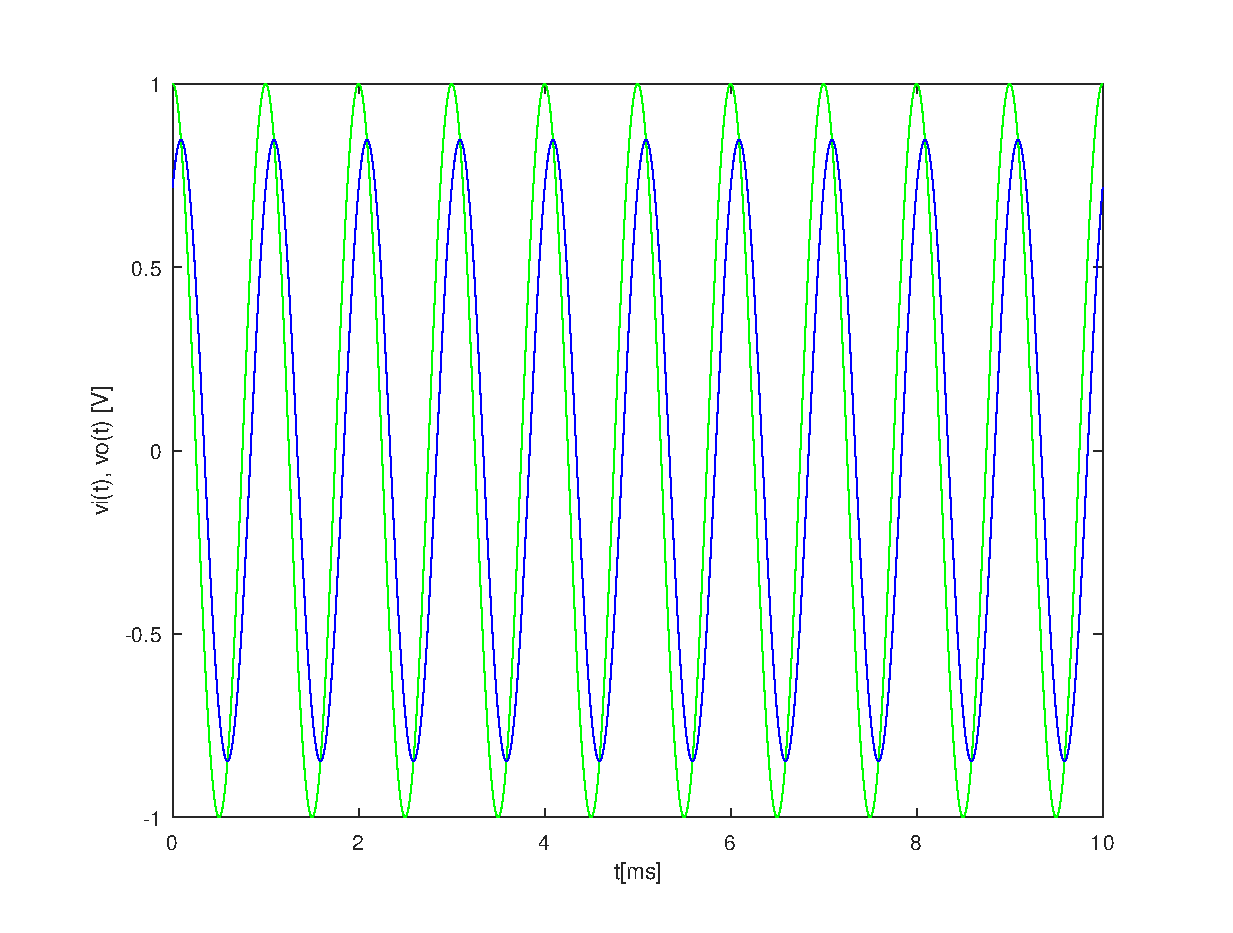
\includegraphics[width=0.8\linewidth]{forced.eps}
\caption{Forced sinusoidal response.}
\label{fig:forced}
\end{figure}

\section{Frequency response}

\lipsum[1-1]




\section{Simulation Analysis}
\label{sec:simulation}

In addition to theoretical analysis, we computed a simulation of the AC/DC converter using Ngspice, and plotted the output voltages of the envelope detector and voltage regulator circuits. The results are illustrated in Figure~\ref{fig:venvout}.

\vspace{-30mm}

\begin{figure}[H] \centering
\includegraphics[width=0.6\linewidth]{../sim/venvout.pdf}
\caption{Plots of the output voltages of the envelope detector (blue) and voltage regulator (red) circuits obtained by simulation.}
\label{fig:venvout}
\end{figure}

So as to observe the deviation of the output signal from 12V, we also plotted the Ngspice reproduction of $v_o-12$, which we can see in Figure~\ref{fig:vdiff}.

\vspace{-20mm}

\begin{figure}[H] \centering
\includegraphics[width=0.6\linewidth]{../sim/vdiff.pdf}
\caption{Deviation of the output signal from 12V obtained by simulation.}
\label{fig:vdiff}
\end{figure}

Furthermore, we managed to determine the average of $v_o$ and its respective ripple. The average deviation from $12V$ and the ripple of the output voltage obtained by simulation are presented in Table~\ref{tab:results}, side by side to the corresponding values obtained previously with Octave.

\vspace{2mm}

\begin{center}
\begin{tabular}{ | c | c | c | }\hline
\input{../mat/simtab} 
\end{tabular}
\captionof{table}[]{Average deviation from $12V$ and ripple of the output voltage obtained theoretically and by simulation.}
\label{tab:results}
\end{center}

\vspace{2mm}

Comparing the theoretical results to the ones obtained by simulation, one notices that the average deviation from 12V is approximately 0 for the first one and exactly 0 for the second one. Similarly, the ripple calculated with Octave is very close to the one computed with Ngspice. With this in mind, and taking into account that the plots presented in both sections match almost precisely, it becomes evident that both methods are in agreement in terms of the obtained results.\\

Finally, to calculate the merit $M$ of the converter, we used the values obtained by simulation. They should be more reliable, since in the theoretical analysis we considered several approximations that may have affected the results. The merit $M$, as well as the values required to its calculation, are illustrated in Table~\ref{tab:merit}.

\vspace{2mm}

\begin{center}
\begin{tabular}{ | c | c | }\hline
\input{../mat/merit} 
\end{tabular}
\captionof{table}[]{Merit of the converter.}
\label{tab:merit}
\end{center}



\section{Conclusion}
\label{sec:conclusion}

In this laboratory assignment the objective of analysing an RC circuit has been
achieved. Static, time and frequency analyses have been performed both
theoretically using the Octave maths tool and by circuit simulation using the
Ngspice tool. The simulation results matched the theoretical results
precisely. The reason for this perfect match is the fact that this is a
straightforward circuit containing only linear components, so the theoretical
and simulation models cannot differ. For more complex components, the
theoretical and simulation models could differ but this is not the case in this
work.

\lipsum[1-1]

%\cleardoublepage

% ----------------------------------------------------------------------
%  Bibliography
% ----------------------------------------------------------------------
%\addcontentsline{toc}{section}{\bibname}
%\bibliographystyle{abbrvunsrtnat} % <<<<< SELECT IF USING REFERENCES BY NUMBER (CITATION ORDER)
%\bibliography{../../../BIBfile.bib}

% ----------------------------------------------------------------------
\end{document}
% ----------------------------------------------------------------------
